% Options for packages loaded elsewhere
\PassOptionsToPackage{unicode}{hyperref}
\PassOptionsToPackage{hyphens}{url}
%
\documentclass[
  man]{apa6}
\usepackage{amsmath,amssymb}
\usepackage{lmodern}
\usepackage{iftex}
\ifPDFTeX
  \usepackage[T1]{fontenc}
  \usepackage[utf8]{inputenc}
  \usepackage{textcomp} % provide euro and other symbols
\else % if luatex or xetex
  \usepackage{unicode-math}
  \defaultfontfeatures{Scale=MatchLowercase}
  \defaultfontfeatures[\rmfamily]{Ligatures=TeX,Scale=1}
\fi
% Use upquote if available, for straight quotes in verbatim environments
\IfFileExists{upquote.sty}{\usepackage{upquote}}{}
\IfFileExists{microtype.sty}{% use microtype if available
  \usepackage[]{microtype}
  \UseMicrotypeSet[protrusion]{basicmath} % disable protrusion for tt fonts
}{}
\makeatletter
\@ifundefined{KOMAClassName}{% if non-KOMA class
  \IfFileExists{parskip.sty}{%
    \usepackage{parskip}
  }{% else
    \setlength{\parindent}{0pt}
    \setlength{\parskip}{6pt plus 2pt minus 1pt}}
}{% if KOMA class
  \KOMAoptions{parskip=half}}
\makeatother
\usepackage{xcolor}
\usepackage{graphicx}
\makeatletter
\def\maxwidth{\ifdim\Gin@nat@width>\linewidth\linewidth\else\Gin@nat@width\fi}
\def\maxheight{\ifdim\Gin@nat@height>\textheight\textheight\else\Gin@nat@height\fi}
\makeatother
% Scale images if necessary, so that they will not overflow the page
% margins by default, and it is still possible to overwrite the defaults
% using explicit options in \includegraphics[width, height, ...]{}
\setkeys{Gin}{width=\maxwidth,height=\maxheight,keepaspectratio}
% Set default figure placement to htbp
\makeatletter
\def\fps@figure{htbp}
\makeatother
\setlength{\emergencystretch}{3em} % prevent overfull lines
\providecommand{\tightlist}{%
  \setlength{\itemsep}{0pt}\setlength{\parskip}{0pt}}
\setcounter{secnumdepth}{-\maxdimen} % remove section numbering
% Make \paragraph and \subparagraph free-standing
\ifx\paragraph\undefined\else
  \let\oldparagraph\paragraph
  \renewcommand{\paragraph}[1]{\oldparagraph{#1}\mbox{}}
\fi
\ifx\subparagraph\undefined\else
  \let\oldsubparagraph\subparagraph
  \renewcommand{\subparagraph}[1]{\oldsubparagraph{#1}\mbox{}}
\fi
\newlength{\cslhangindent}
\setlength{\cslhangindent}{1.5em}
\newlength{\csllabelwidth}
\setlength{\csllabelwidth}{3em}
\newlength{\cslentryspacingunit} % times entry-spacing
\setlength{\cslentryspacingunit}{\parskip}
\newenvironment{CSLReferences}[2] % #1 hanging-ident, #2 entry spacing
 {% don't indent paragraphs
  \setlength{\parindent}{0pt}
  % turn on hanging indent if param 1 is 1
  \ifodd #1
  \let\oldpar\par
  \def\par{\hangindent=\cslhangindent\oldpar}
  \fi
  % set entry spacing
  \setlength{\parskip}{#2\cslentryspacingunit}
 }%
 {}
\usepackage{calc}
\newcommand{\CSLBlock}[1]{#1\hfill\break}
\newcommand{\CSLLeftMargin}[1]{\parbox[t]{\csllabelwidth}{#1}}
\newcommand{\CSLRightInline}[1]{\parbox[t]{\linewidth - \csllabelwidth}{#1}\break}
\newcommand{\CSLIndent}[1]{\hspace{\cslhangindent}#1}
\ifLuaTeX
\usepackage[bidi=basic]{babel}
\else
\usepackage[bidi=default]{babel}
\fi
\babelprovide[main,import]{english}
% get rid of language-specific shorthands (see #6817):
\let\LanguageShortHands\languageshorthands
\def\languageshorthands#1{}
% Manuscript styling
\usepackage{upgreek}
\captionsetup{font=singlespacing,justification=justified}

% Table formatting
\usepackage{longtable}
\usepackage{lscape}
% \usepackage[counterclockwise]{rotating}   % Landscape page setup for large tables
\usepackage{multirow}		% Table styling
\usepackage{tabularx}		% Control Column width
\usepackage[flushleft]{threeparttable}	% Allows for three part tables with a specified notes section
\usepackage{threeparttablex}            % Lets threeparttable work with longtable

% Create new environments so endfloat can handle them
% \newenvironment{ltable}
%   {\begin{landscape}\centering\begin{threeparttable}}
%   {\end{threeparttable}\end{landscape}}
\newenvironment{lltable}{\begin{landscape}\centering\begin{ThreePartTable}}{\end{ThreePartTable}\end{landscape}}

% Enables adjusting longtable caption width to table width
% Solution found at http://golatex.de/longtable-mit-caption-so-breit-wie-die-tabelle-t15767.html
\makeatletter
\newcommand\LastLTentrywidth{1em}
\newlength\longtablewidth
\setlength{\longtablewidth}{1in}
\newcommand{\getlongtablewidth}{\begingroup \ifcsname LT@\roman{LT@tables}\endcsname \global\longtablewidth=0pt \renewcommand{\LT@entry}[2]{\global\advance\longtablewidth by ##2\relax\gdef\LastLTentrywidth{##2}}\@nameuse{LT@\roman{LT@tables}} \fi \endgroup}

% \setlength{\parindent}{0.5in}
% \setlength{\parskip}{0pt plus 0pt minus 0pt}

% Overwrite redefinition of paragraph and subparagraph by the default LaTeX template
% See https://github.com/crsh/papaja/issues/292
\makeatletter
\renewcommand{\paragraph}{\@startsection{paragraph}{4}{\parindent}%
  {0\baselineskip \@plus 0.2ex \@minus 0.2ex}%
  {-1em}%
  {\normalfont\normalsize\bfseries\itshape\typesectitle}}

\renewcommand{\subparagraph}[1]{\@startsection{subparagraph}{5}{1em}%
  {0\baselineskip \@plus 0.2ex \@minus 0.2ex}%
  {-\z@\relax}%
  {\normalfont\normalsize\itshape\hspace{\parindent}{#1}\textit{\addperi}}{\relax}}
\makeatother

% \usepackage{etoolbox}
\makeatletter
\patchcmd{\HyOrg@maketitle}
  {\section{\normalfont\normalsize\abstractname}}
  {\section*{\normalfont\normalsize\abstractname}}
  {}{\typeout{Failed to patch abstract.}}
\patchcmd{\HyOrg@maketitle}
  {\section{\protect\normalfont{\@title}}}
  {\section*{\protect\normalfont{\@title}}}
  {}{\typeout{Failed to patch title.}}
\makeatother

\usepackage{xpatch}
\makeatletter
\xapptocmd\appendix
  {\xapptocmd\section
    {\addcontentsline{toc}{section}{\appendixname\ifoneappendix\else~\theappendix\fi\\: #1}}
    {}{\InnerPatchFailed}%
  }
{}{\PatchFailed}
\keywords{keywords}
\DeclareDelayedFloatFlavor{ThreePartTable}{table}
\DeclareDelayedFloatFlavor{lltable}{table}
\DeclareDelayedFloatFlavor*{longtable}{table}
\makeatletter
\renewcommand{\efloat@iwrite}[1]{\immediate\expandafter\protected@write\csname efloat@post#1\endcsname{}}
\makeatother
\usepackage{csquotes}
\ifLuaTeX
  \usepackage{selnolig}  % disable illegal ligatures
\fi
\IfFileExists{bookmark.sty}{\usepackage{bookmark}}{\usepackage{hyperref}}
\IfFileExists{xurl.sty}{\usepackage{xurl}}{} % add URL line breaks if available
\urlstyle{same} % disable monospaced font for URLs
\hypersetup{
  pdftitle={How do expert pianists adapt their didactic demonstration to novices' skill levels?},
  pdfauthor={Atsuko Tominaga1, Günther Knoblich1, \& Natalie Sebanz1},
  pdflang={en-EN},
  pdfkeywords={keywords},
  hidelinks,
  pdfcreator={LaTeX via pandoc}}

\title{How do expert pianists adapt their didactic demonstration to novices' skill levels?}
\author{Atsuko Tominaga\textsuperscript{1}, Günther Knoblich\textsuperscript{1}, \& Natalie Sebanz\textsuperscript{1}}
\date{}


\shorttitle{How do expert pianists adapt their didactic demonstration to novices' skill levels?}

\authornote{

Correspondence concerning this article should be addressed to Atsuko Tominaga, Quellenstraße 51, 1100 Vienna, Austria. E-mail: \href{mailto:tominaga_atsuko@phd.ceu.edu}{\nolinkurl{tominaga\_atsuko@phd.ceu.edu}}

}

\affiliation{\vspace{0.5cm}\textsuperscript{1} Department of Cognitive Science, Central European University}

\abstract{%
Later
}



\begin{document}
\maketitle

\hypertarget{introduction}{%
\section{Introduction}\label{introduction}}

\hypertarget{methods}{%
\subsection{Methods}\label{methods}}

\hypertarget{participants}{%
\subsection{Participants}\label{participants}}

We recruited 20 participants who already had a degree (above bachelor's or equivalent) in piano performance/teaching or were studying advanced piano performance at a music school. Most participants were right-handed (left: 2, ambidextrous: 2). The mean age of the participants was 28.25 years (\emph{SD} = 10.95). They had 21.55 years of practice on average (\emph{SD} = 11.59). 17 participants had teaching experience in piano (\emph{M} = 7 years, \emph{SD} = 6.68). All participants were recruited through an online participant platform (SONA system, \url{https://www.sona-systems.com}). The study (No.~2020\_05) was approved by the Psychological Research Ethics Board (PREBO) CEU PU in Austria.

\hypertarget{apparatus-and-stimuli}{%
\subsection{Apparatus and stimuli}\label{apparatus-and-stimuli}}

The experiment was programmed in Max/MSP (8.1.11; \url{https://cycling74.com/products/max}) on a Mac Book Pro with Mac OS X Catalina 10.15.7. A weighted Yamaha MIDI digital piano was used to record participants' performances. The pitch, onset and offset time of each note, and key velocity profiles were obtained from MIDI data using Max/MSP patchers. All auditory feedback was given to participants through headphones (Audio-Technica ATH-M50X). Sheet music was displayed on a computer monitor in front of the participants.

As stimuli, one piece of music, which was used in our previous experiment, was selected (for details, Tominaga et al., 2022). The piece was taken from Clementi's Sonatina Op.36 (No.3) in C major. The first 12 measures of the original piece were used and modified so that the piece had an almost equal number of data points for each dependent variable. The modified piece consisted of a 12-measure isochronous melody notated in 4/4 meter to be played with the right hand only. Two expressive notations (i.e., articulation and dynamics) were added as \emph{Fig \ref{fig:stim}}.

We created artificial recordings of students to manipulate their skill levels. In this experiment, we made the recordings by changing two factors of articulation (present or absent) and dynamics (present or absent). Therefore, there were four types of recordings. We aimed to create a quarter of the recordings where both articulation and dynamics were implemented. The second quarter included the recordings where only articulation was implemented whereas dynamics was missing. The third quarter included the recordings where only dynamics was implemented whereas articulation was missing. The last quarter included the recordings where neither articulation nor dynamics was implemented. We generated 4 instances for each type, therefore there were 16 stimuli (i.e., recordings) in total. How we generated the stimuli is written in \emph{Supplementary Material}.

\begin{figure}
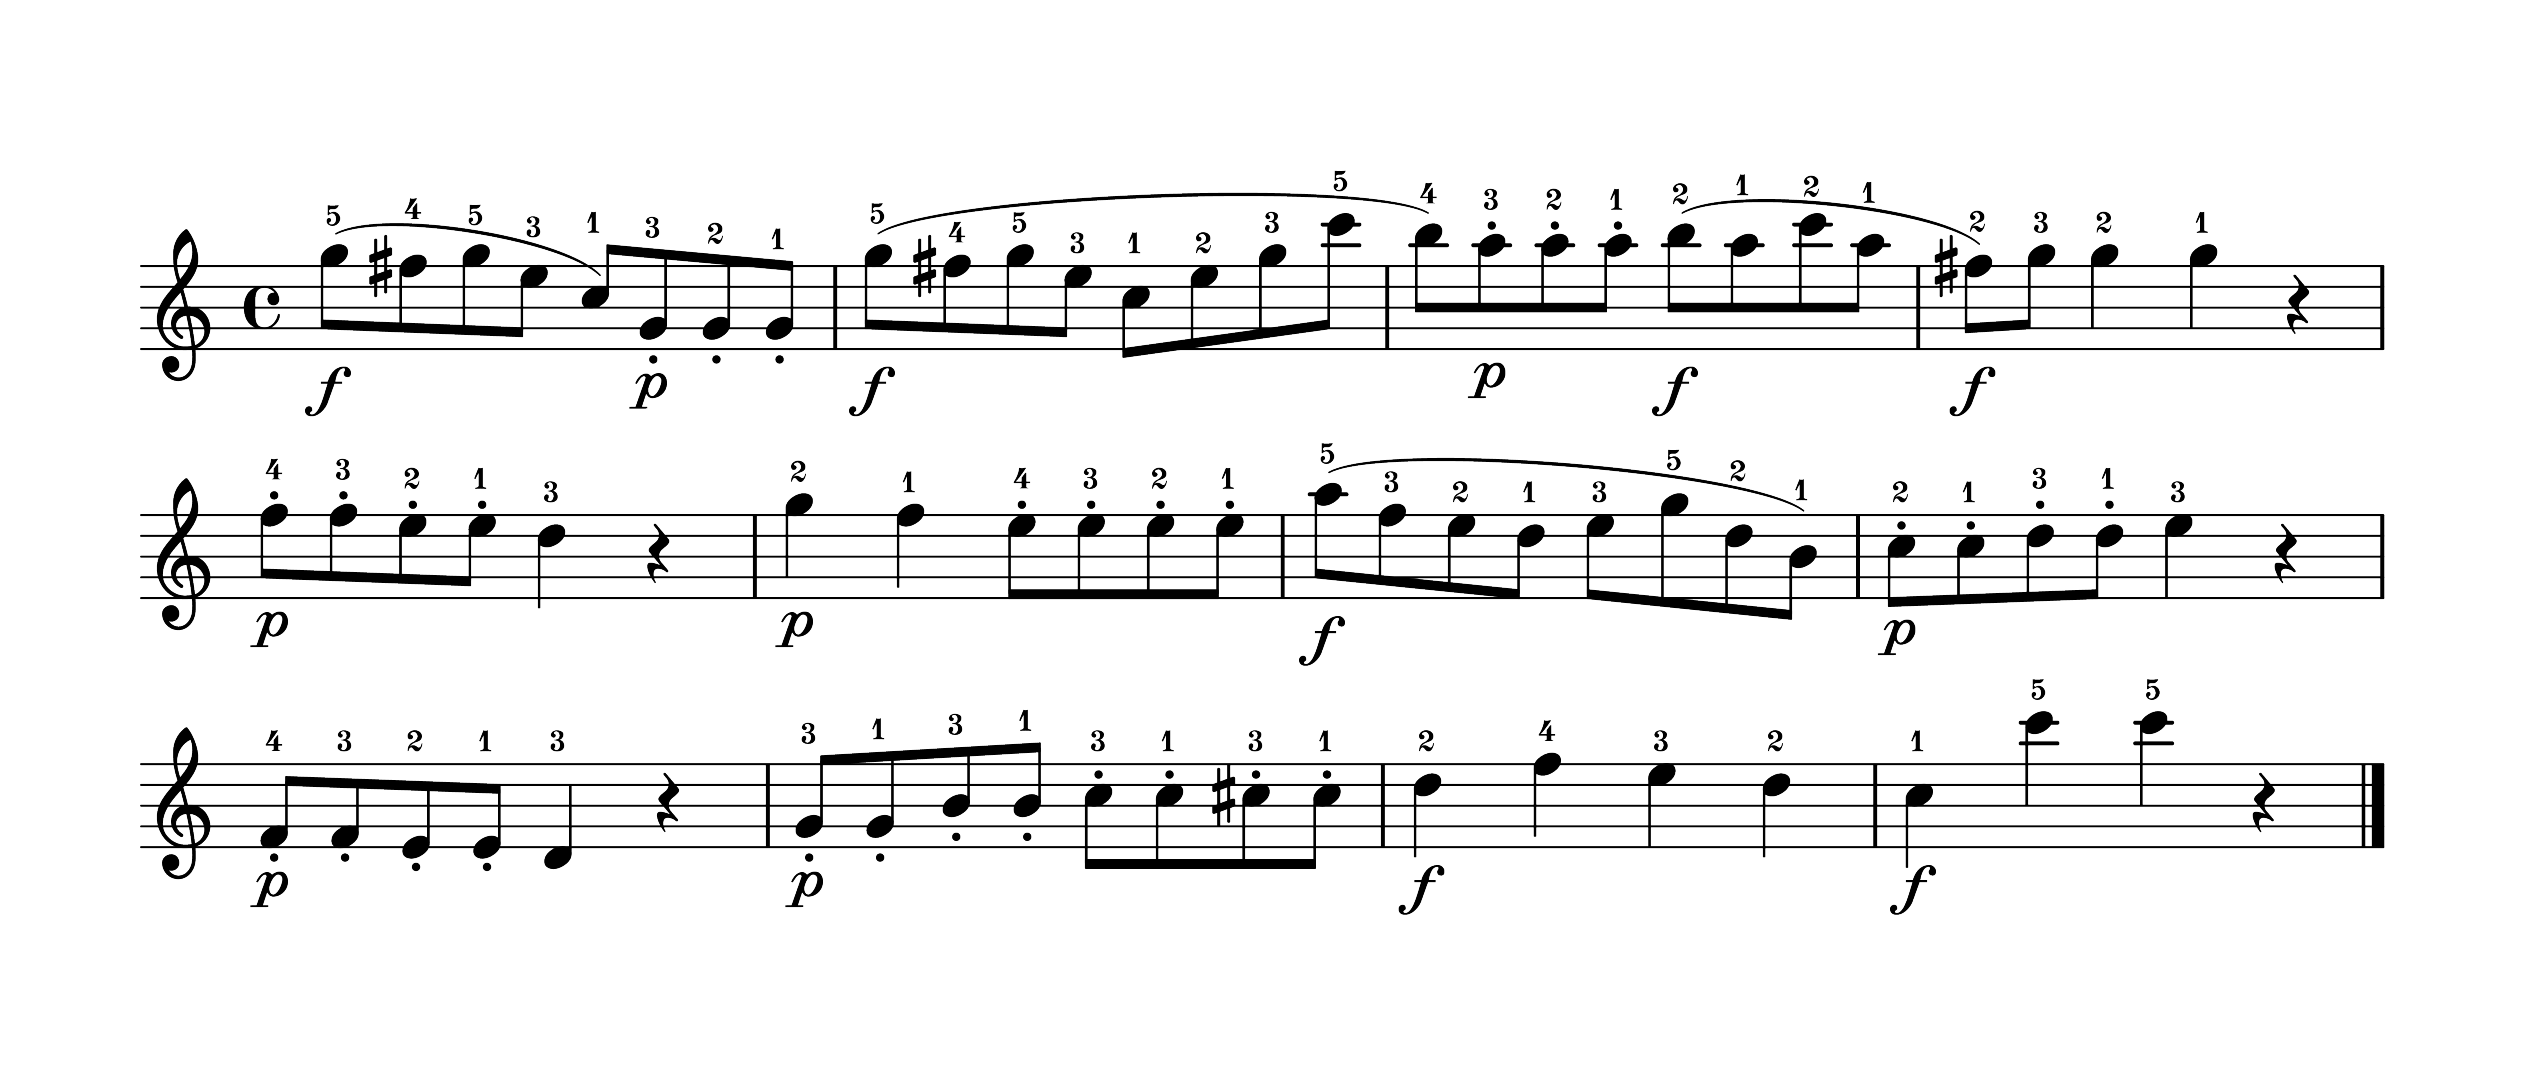
\includegraphics[width=1\linewidth]{manuscript_files/figure-latex/stimli-1} \caption{\label{fig:stim}Sheet music. Articulation. For articulation notation, the curved line (slur) indicates legato and the dots indicate staccato. For dynamics notation, the symbol `f' denotes forte and the symbol `p' denotes piano. For data analysis, only the 8th notes were included.}\label{fig:stimli}
\end{figure}

\hypertarget{procedure}{%
\subsection{Procedure}\label{procedure}}

Prior to the experiment, participants were required to memorise the piece so that they had enough time to practise and perform it without pitch errors while implementing notated expressions in the experiment.

First, we recorded participants' baseline performance by asking them to perform the piece without listening to any students' performance. A leading metronome (100 quarter beats per minute, 8 beats) was given before participants started performing the piece. Sheet music (\emph{Fig \ref{fig:stim}}) was displayed in front of the participants. Also, they were told to perform the piece expressively with their interpretation and do their best as a performer. This instruction was given to make sure that they paid attention to expressive aspects of the performance. Each participant performed the piece twice.

After we recorded the participants' baseline performance, participants were informed that they were going to listen to a number of recordings from 16 different students, who were learning musical expressive techniques. Participants were required to listen to each student's recording first, and then to perform the same piece to teach musical expressive techniques to the student (i.e., recording). In total, there were 16 trials and participants played the piece for each recording only once. The order of the recordings was randomised for each participant. A leading metronome (100 quarter beats per minute, 8 beats) was given before participants started performing the piece.

After participants completed the 16 trials, they were asked to perform the piece in the same situation as we recorded their baseline performance. At the end of the experiment, participants filled in a questionnaire asking about their demographic information and experience in piano performance/teaching.

\hypertarget{data-analysis}{%
\subsection{Data analysis}\label{data-analysis}}

The dependent variables were computed from MIDI data for data analysis. Interonset intervals (IOIs) are the intervals between onsets of adjacent notes and provide a measure of tempo. Key-overlap time (KOT) is the difference between the offset time of the current tone (i.e., key release time) and the onset time of the ensuing tone and is a measure for the smoothness of musical sequences. A positive value indicates smooth legato styles due to overlap between the current and ensuing tone whereas a negative value indicates sharp staccato styles due to separation between the current and ensuing note. Tone intensity is assessed by key velocity (KV) and measures the loudness of a musical note. A higher value indicates forte styles whereas a lower value indicates piano styles. The value of KV in MIDI varies between 0 (minimum) and 127 (maximum). Also, KV difference was calculated by subtracting the KV value of the current note from that of the following note. We particularly focused on specific points where each subcomponent changed from one to the other (i.e., forte to piano or piano to forte) to measure dynamics contrast between forte and piano.

Data processing and statistical analysis were performed in R version 4.0.5. For statistical analysis, we included 8th notes with expressive notations only. Pitch errors were identified by comparing the sequence of musical notes produced by a participant with the sequence of musical notes according to the sheet music. Pitch errors included either, extra, missing or substituted tones and were manually removed by using the \emph{editData} R package. For note onsets, 31.87 \% of the trials contained at least one pitch error (extra notes: 5.94 \%, missing notes: 24.38 \%, substituted notes: 1.56 \%). For note offsets, 35.31 \% of the trials contained at least one pitch error (extra notes: 5.94 \%, missing notes: 24.38 \%, substituted notes: 5 \%). We found that some participants did not precisely follow the sheet music (e.g., they held some notes longer than notated), therefore the order of offsets did not correspond to that of onsets. We considered these as errors and removed the erroneous notes even if the order of onsets was correct. As a result, less than 1 \% of total responses were corrected. After removing pitch errors, we removed outliers for IOIs, KOT, KV and KV Difference, defined as values more than 3 standard deviations from the mean of each dependent variable. For each dependent variable, this resulted in less than 2 \% of overall responses being removed as outliers.

We performed a 2 x 2 repeated-measures analysis of variance (ANOVA) with the factors Articulation (present vs.~absent) and Dynamics (present or absent) for each dependent variable (i.e.., IOIs, KOT, KV, KV Difference). The \emph{aov\_ez} function in the \emph{afex} R package was used for a repeated-measures ANOVA. For post-doc comparisons on the estimated marginal means, we used the \emph{emmeans} R package.

\hypertarget{results}{%
\section{Results}\label{results}}

All effects are reported as significant at \emph{p} \textless{} .05. For KOT, KV and KV Difference, we performed two-way ANOVAs separately for each subcomponent (i.e., legato, staccato, forte, piano).

\hypertarget{iois}{%
\subsection{IOIs}\label{iois}}

Neither main effect of Articulation (\emph{F}(1, 19) = 2.79, \emph{p} = 0.111, \(\eta_G^2\) = 0.010) or Dynamics (\emph{F}(1, 19) = 3.27, \emph{p} = 0.086, \(\eta_G^2\) = 0.003) nor the interaction between Articulation and Dynamics was significant (\emph{F}(1, 19) = 1.48, \emph{p} = 0.24, \(\eta_G^2\) = 0.002). Therefore, participants did not change the tempo depending on the types of the recordings (\emph{Fig \ref{fig:ioi-1}}).

\hypertarget{kot}{%
\subsection{KOT}\label{kot}}

\hypertarget{legato}{%
\subsubsection{Legato}\label{legato}}

There was a significant main effect of Articulation (\emph{F}(1, 19) = 5.59, \emph{p} = 0.029, \(\eta_G^2\) = 0.002). However, there was no significant main effect of Dynamics (\emph{F}(1, 19) = 0.06, \emph{p} = 0.81, \(\eta_G^2\) = 0.000) or interaction between Articulation and Dynamics (\emph{F}(1, 19) = 1.89, \emph{p} = 0.19, \(\eta_G^2\) = 0.002). Participants produced longer legato when listening to the recordings where articulation was not implemented (\emph{Fig \ref{fig:kot-1}}, left).

\hypertarget{staccato}{%
\subsubsection{Staccato}\label{staccato}}

There was a significant main effect of Articulation (\emph{F}(1, 19) = 4.88, \emph{p} = 0.040, \(\eta_G^2\) = 0.009). However, there was no significant main effect of Dynamics (\emph{F}(1, 19) = 0.68, \emph{p} = 0.42, \(\eta_G^2\) = 0.000) or interaction between Articulation and Dynamics (\emph{F}(1, 19) = 3.13, \emph{p} = 0.093, \(\eta_G^2\) = 0.001). Participants produced shorter staccato when listening to the recordings where articulation was not implemented (\emph{Fig \ref{fig:kot-1}}, right).

\hypertarget{kv}{%
\subsection{KV}\label{kv}}

\hypertarget{forte}{%
\subsubsection{Forte}\label{forte}}

Neither main effect of Articulation (\emph{F}(1, 19) = 1.66, \emph{p} = 0.213, \(\eta_G^2\) = 0.00) or Dynamics (\emph{F}(1, 19) = 0.33, \emph{p} = 0.57, \(\eta_G^2\) = 0.000) nor the interaction between Articulation and Dynamics was significant (\emph{F}(1, 19) = 0.00, \emph{p} = 0.96, \(\eta_G^2\) = 0.000). Participants did not change performances in terms of dynamics (loudness) depending on the types of the recordings (\emph{Fig \ref{fig:vel-1}}, left).

\hypertarget{piano}{%
\subsubsection{Piano}\label{piano}}

There was a significant main effect of Articulation (\emph{F}(1, 19) = 7.18, \emph{p} = 0.01, \(\eta_G^2\) = 0.060). However, there was no significant main effect of Dynamics (\emph{F}(1, 19) = 1.80, \emph{p} = 0.20, \(\eta_G^2\) = 0.003) or interaction between Articulation and Dynamics (\emph{F}(1, 19) = 0.04, \emph{p} = 0.85, \(\eta_G^2\) = 0.000). Participants produced softer piano when listening to the recordings where articulation was implemented (\emph{Fig \ref{fig:vel-1}}, right).

\hypertarget{kv-difference}{%
\subsection{KV Difference}\label{kv-difference}}

\hypertarget{forte-to-piano}{%
\subsubsection{Forte to Piano}\label{forte-to-piano}}

Neither main effect of Articulation (\emph{F}(1, 19) = 3.40, \emph{p} = 0.081, \(\eta_G^2\) = 0.012) or Dynamics (\emph{F}(1, 19) = 1.58, \emph{p} = 0.22, \(\eta_G^2\) = 0.002) nor the interaction between Articulation and Dynamics was significant (\emph{F}(1, 19) = 0.97, \emph{p} = 0.336, \(\eta_G^2\) = 0.001).

\hypertarget{piano-to-forte}{%
\subsubsection{Piano to Forte}\label{piano-to-forte}}

Neither main effect of Articulation (\emph{F}(1, 19) = 2.25, \emph{p} = 0.150, \(\eta_G^2\) = 0.005) or Dynamics (\emph{F}(1, 19) = 3.76, \emph{p} = 0.07, \(\eta_G^2\) = 0.004) nor the interaction between Articulation and Dynamics was significant (\emph{F}(1, 19) = 1.08, \emph{p} = 0.31, \(\eta_G^2\) = 0.001).

These results indicated that participants did not change performances in terms of dynamics contrast depending on the types of the recording (\emph{Fig \ref{fig:vel-diff-1}}).

\begin{figure}
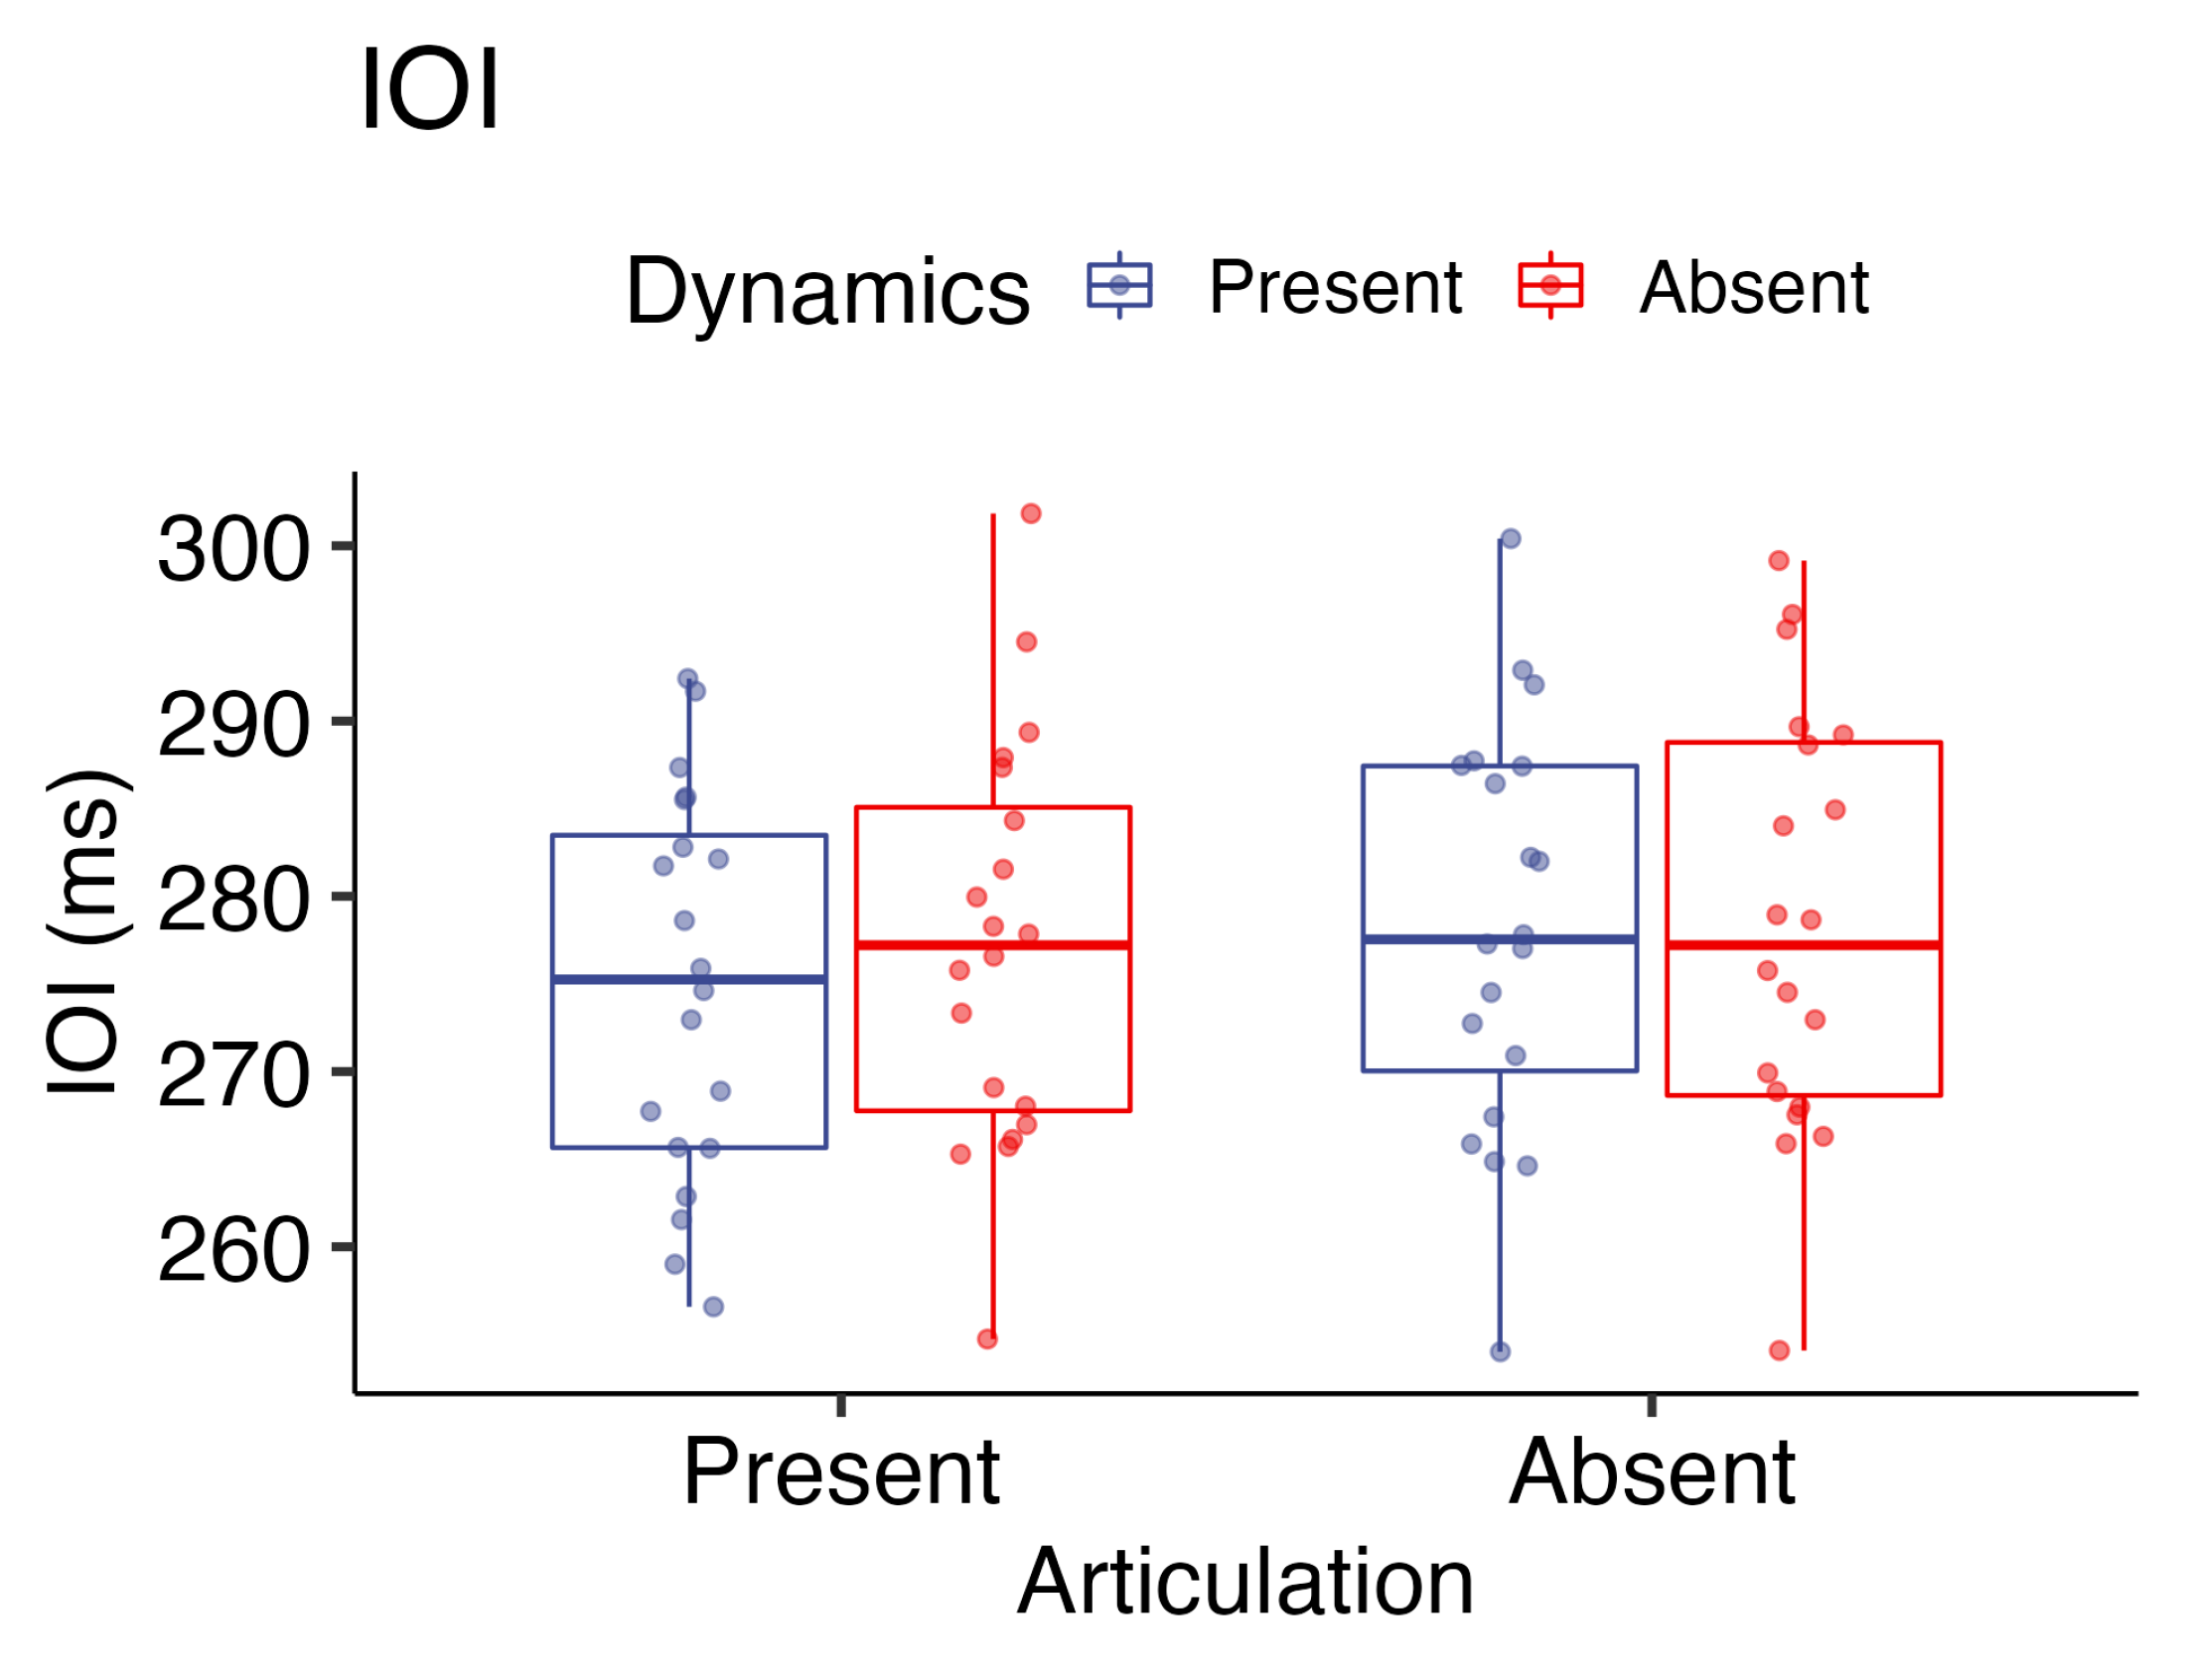
\includegraphics[width=1\linewidth]{manuscript_files/figure-latex/plot-ioi-1-1} \caption{\label{fig:ioi-1}IOIs (ms). Each box indicates the IQR with the median, and whiskers extend to a maximum of 1.5 × IQR beyond the box.}\label{fig:plot-ioi-1}
\end{figure}

\begin{figure}
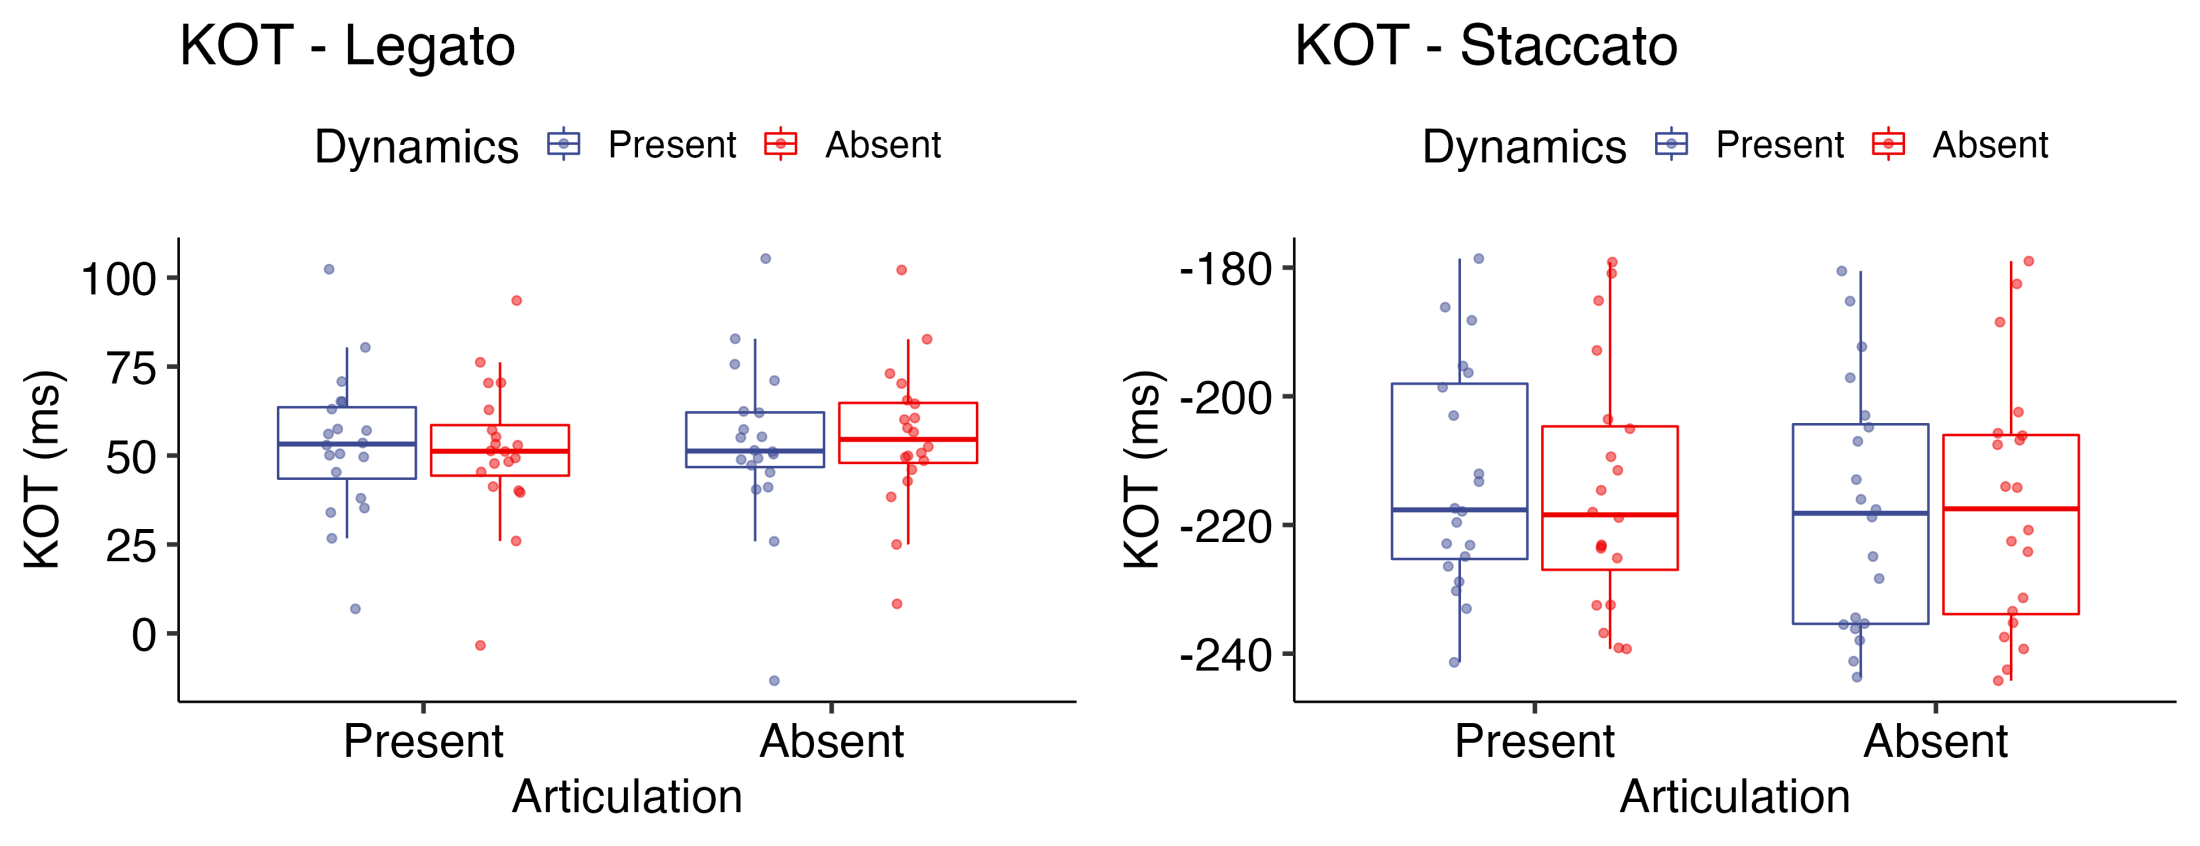
\includegraphics[width=1\linewidth]{manuscript_files/figure-latex/plot-kot-1-1} \caption{\label{fig:kot-1}KOT(ms) for each subcomponent; legato (left) and staccato (right). Each box indicates the IQR with the median, and whiskers extend to a maximum of 1.5 × IQR beyond the box.}\label{fig:plot-kot-1}
\end{figure}

\begin{figure}
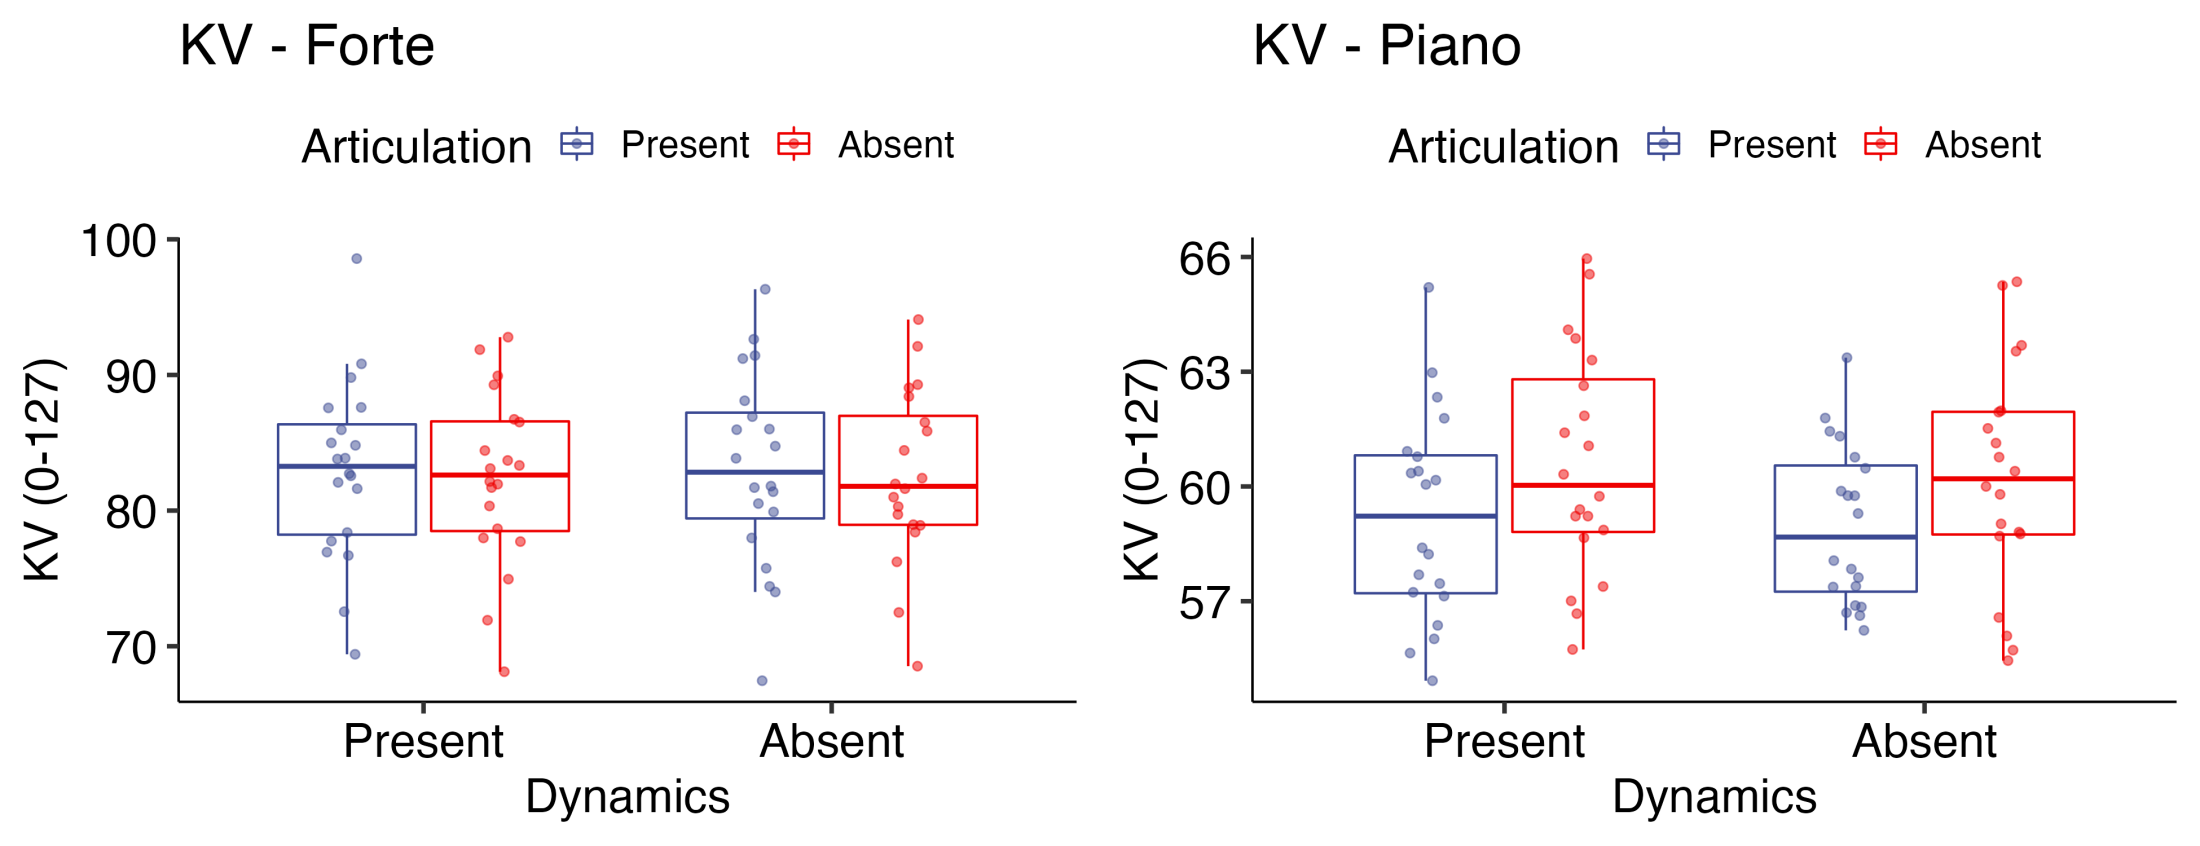
\includegraphics[width=1\linewidth]{manuscript_files/figure-latex/plot-vel-1-1} \caption{\label{fig:vel-1}KV (0-127) for each subcomponent; forte (left) and piano (right). Each box indicates the IQR with the median, and whiskers extend to a maximum of 1.5 × IQR beyond the box.}\label{fig:plot-vel-1}
\end{figure}

\begin{figure}
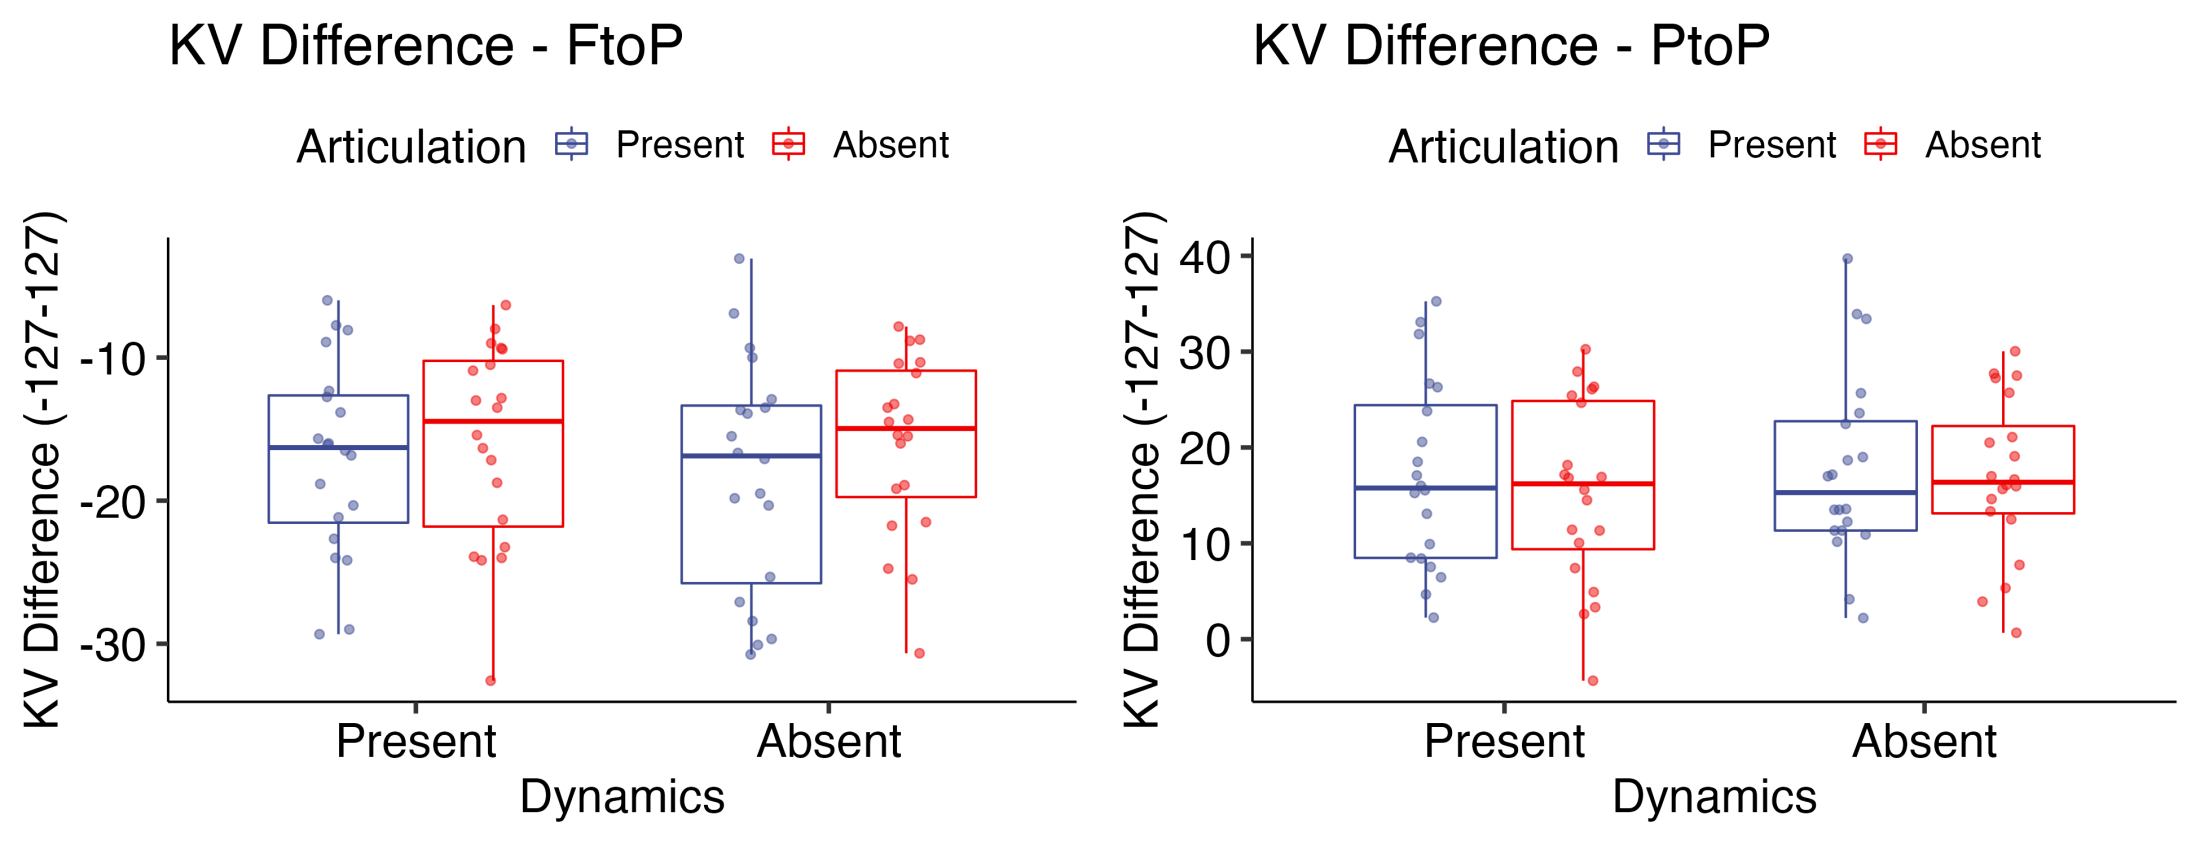
\includegraphics[width=1\linewidth]{manuscript_files/figure-latex/plot-vel-diff-1-1} \caption{\label{fig:vel-diff-1}KV Difference (-127-127) for each subcomponent; forte to piano (left) and piano to forte (right). Each box indicates the IQR with the median, and whiskers extend to a maximum of 1.5 × IQR beyond the box.}\label{fig:plot-vel-diff-1}
\end{figure}

\hypertarget{comparison-with-baseline-performance}{%
\subsection{Comparison with baseline performance}\label{comparison-with-baseline-performance}}

In order to investigate how their performances during the experiment differed from their baseline performances (i.e., performances that participants produced before listening to any of the recordings), we performed one-way repeated-measures ANOVAs. For KOT, KV and KV Difference, we performed ANOVAs separately for each subcomponent. To recall the instruction for the baseline performance, we asked participants to perform the piece expressively with their interpretation and do their best as a performer. By comparing with the baseline performance, we can investigate how didactic intentions influence participants' performances.

\hypertarget{iois-1}{%
\subsection{IOIs}\label{iois-1}}

We compared the baseline performance with the performances where either both articulation and dynamics were implemented or neither of them was implemented to examine how participants performed differently for these extreme examples of students' skill levels. We categorised performances into three groups (baseline, both, none) and treated them as a factor Category.

There was no significant main effect of Category (\emph{F}(1.11, 21.18) = 0.58, \emph{p} = 0.47, \(\eta_G^2\) = 0.012; Greenhouse-Geisser corrected), suggesting that participants kept the same tempo regardless of whether they had an intention to teach (\emph{Fig \ref{fig:ioi-2}}).

\hypertarget{kot-1}{%
\subsection{KOT}\label{kot-1}}

We compared the baseline performance with the performances where dynamics was implemented to examine how participants performed differently depending on whether articulation was implemented or not on each recording. We categorised performances into three groups (baseline, both (i.e., articulation-present, dynamics-present), dynamics-only (i.e., articulation-absent, dynamics-present)) and treated them as a factor Category.

\hypertarget{legato-1}{%
\subsubsection{Legato}\label{legato-1}}

There was a significant main effect of Category (\emph{F}(1.45, 27.53) = 11.82, \emph{p} \textless{} 0.001, \(\eta_G^2\) = 0.060; Greenhouse-Geisser corrected). Post-hoc comparisons based on the estimated marginal means with Tukey adjustment showed that there were differences between baseline and the other two categories (baseline and both: \emph{p} \textless{} .001 , baseline and dynamics-only: \emph{p} .008), suggesting that participants produced longer legato when they had an intention to teach (\emph{Fig \ref{fig:kot-2}}, left).

\hypertarget{staccato-1}{%
\subsubsection{Staccato}\label{staccato-1}}

There was no significant main effect of Category (\emph{F}(1.12, 21.28) = 0.75, \emph{p} = 0.41, \(\eta_G^2\) = 0.011; Greenhouse-Geisser corrected), suggesting that participants did not play staccato differently depending on whether they had an intention to teach (\emph{Fig \ref{fig:kot-2}}, right).

\hypertarget{kv-1}{%
\subsection{KV}\label{kv-1}}

We compared the baseline performance with the performances where articulation was implemented to examine how participants performed differently depending on whether dynamics was implemented or not on each recording. We categorised performances into three groups (baseline, both (i.e., articulation-present, dynamics-present), articulation-only (i.e., articulation-present, dynamics-absent)) and treated them as a factor Category.

\hypertarget{forte-1}{%
\subsubsection{Forte}\label{forte-1}}

There was no significant main effect of Category (\emph{F}(1.59, 30.18) = 1.43, \emph{p} = 0.25, \(\eta_G^2\) = 0.004; Greenhouse-Geisser corrected), suggesting that participants did not play forte differently depending on whether they had an intention to teach (\emph{Fig \ref{fig:vel-2}}, left).

\hypertarget{piano-1}{%
\subsubsection{Piano}\label{piano-1}}

There was a significant main effect of Category (\emph{F}(1.79, 34.09) = 5.68, \emph{p} = 0.009, \(\eta_G^2\) = 0.072; Greenhouse-Geisser corrected). Post-hoc comparisons based on the estimated marginal means with Tukey adjustment showed that there were differences between baseline and the other two categories (baseline and both: \emph{p} .05 , baseline and articulation-only: \emph{p} .03), suggesting that participants produced softer piano when they had an intention to teach (\emph{Fig \ref{fig:vel-2}}, right).

\hypertarget{kv-difference-1}{%
\subsection{KV Difference}\label{kv-difference-1}}

We compared the baseline performance with the performances where articulation was implemented to examine how participants performed differently depending on whether dynamics was implemented or not on each recording. We categorised performances into three groups (baseline, both (i.e., articulation-present, dynamics-present), articulation-only (i.e., articulation-present, dynamics-absent)) and treated them as a factor Category.

\hypertarget{forte-to-piano-1}{%
\subsubsection{Forte to Piano}\label{forte-to-piano-1}}

There was no significant main effect of Category (\emph{F}(1.53, 29.15) = 1.73, \emph{p} = 0.20, \(\eta_G^2\) = 0.014; Greenhouse-Geisser corrected).

\hypertarget{piano-to-forte-1}{%
\subsubsection{Piano to Forte}\label{piano-to-forte-1}}

There was no significant main effect of Category (\emph{F}(1.28, 24.39) = 2.27, \emph{p} = 0.14, \(\eta_G^2\) = 0.013; Greenhouse-Geisser corrected).

These results indicated that participants did not make dynamics contrast between forte and piano differently depending on whether they had an intention to teach (\emph{Fig \ref{fig:vel-diff-2}}).

\begin{figure}
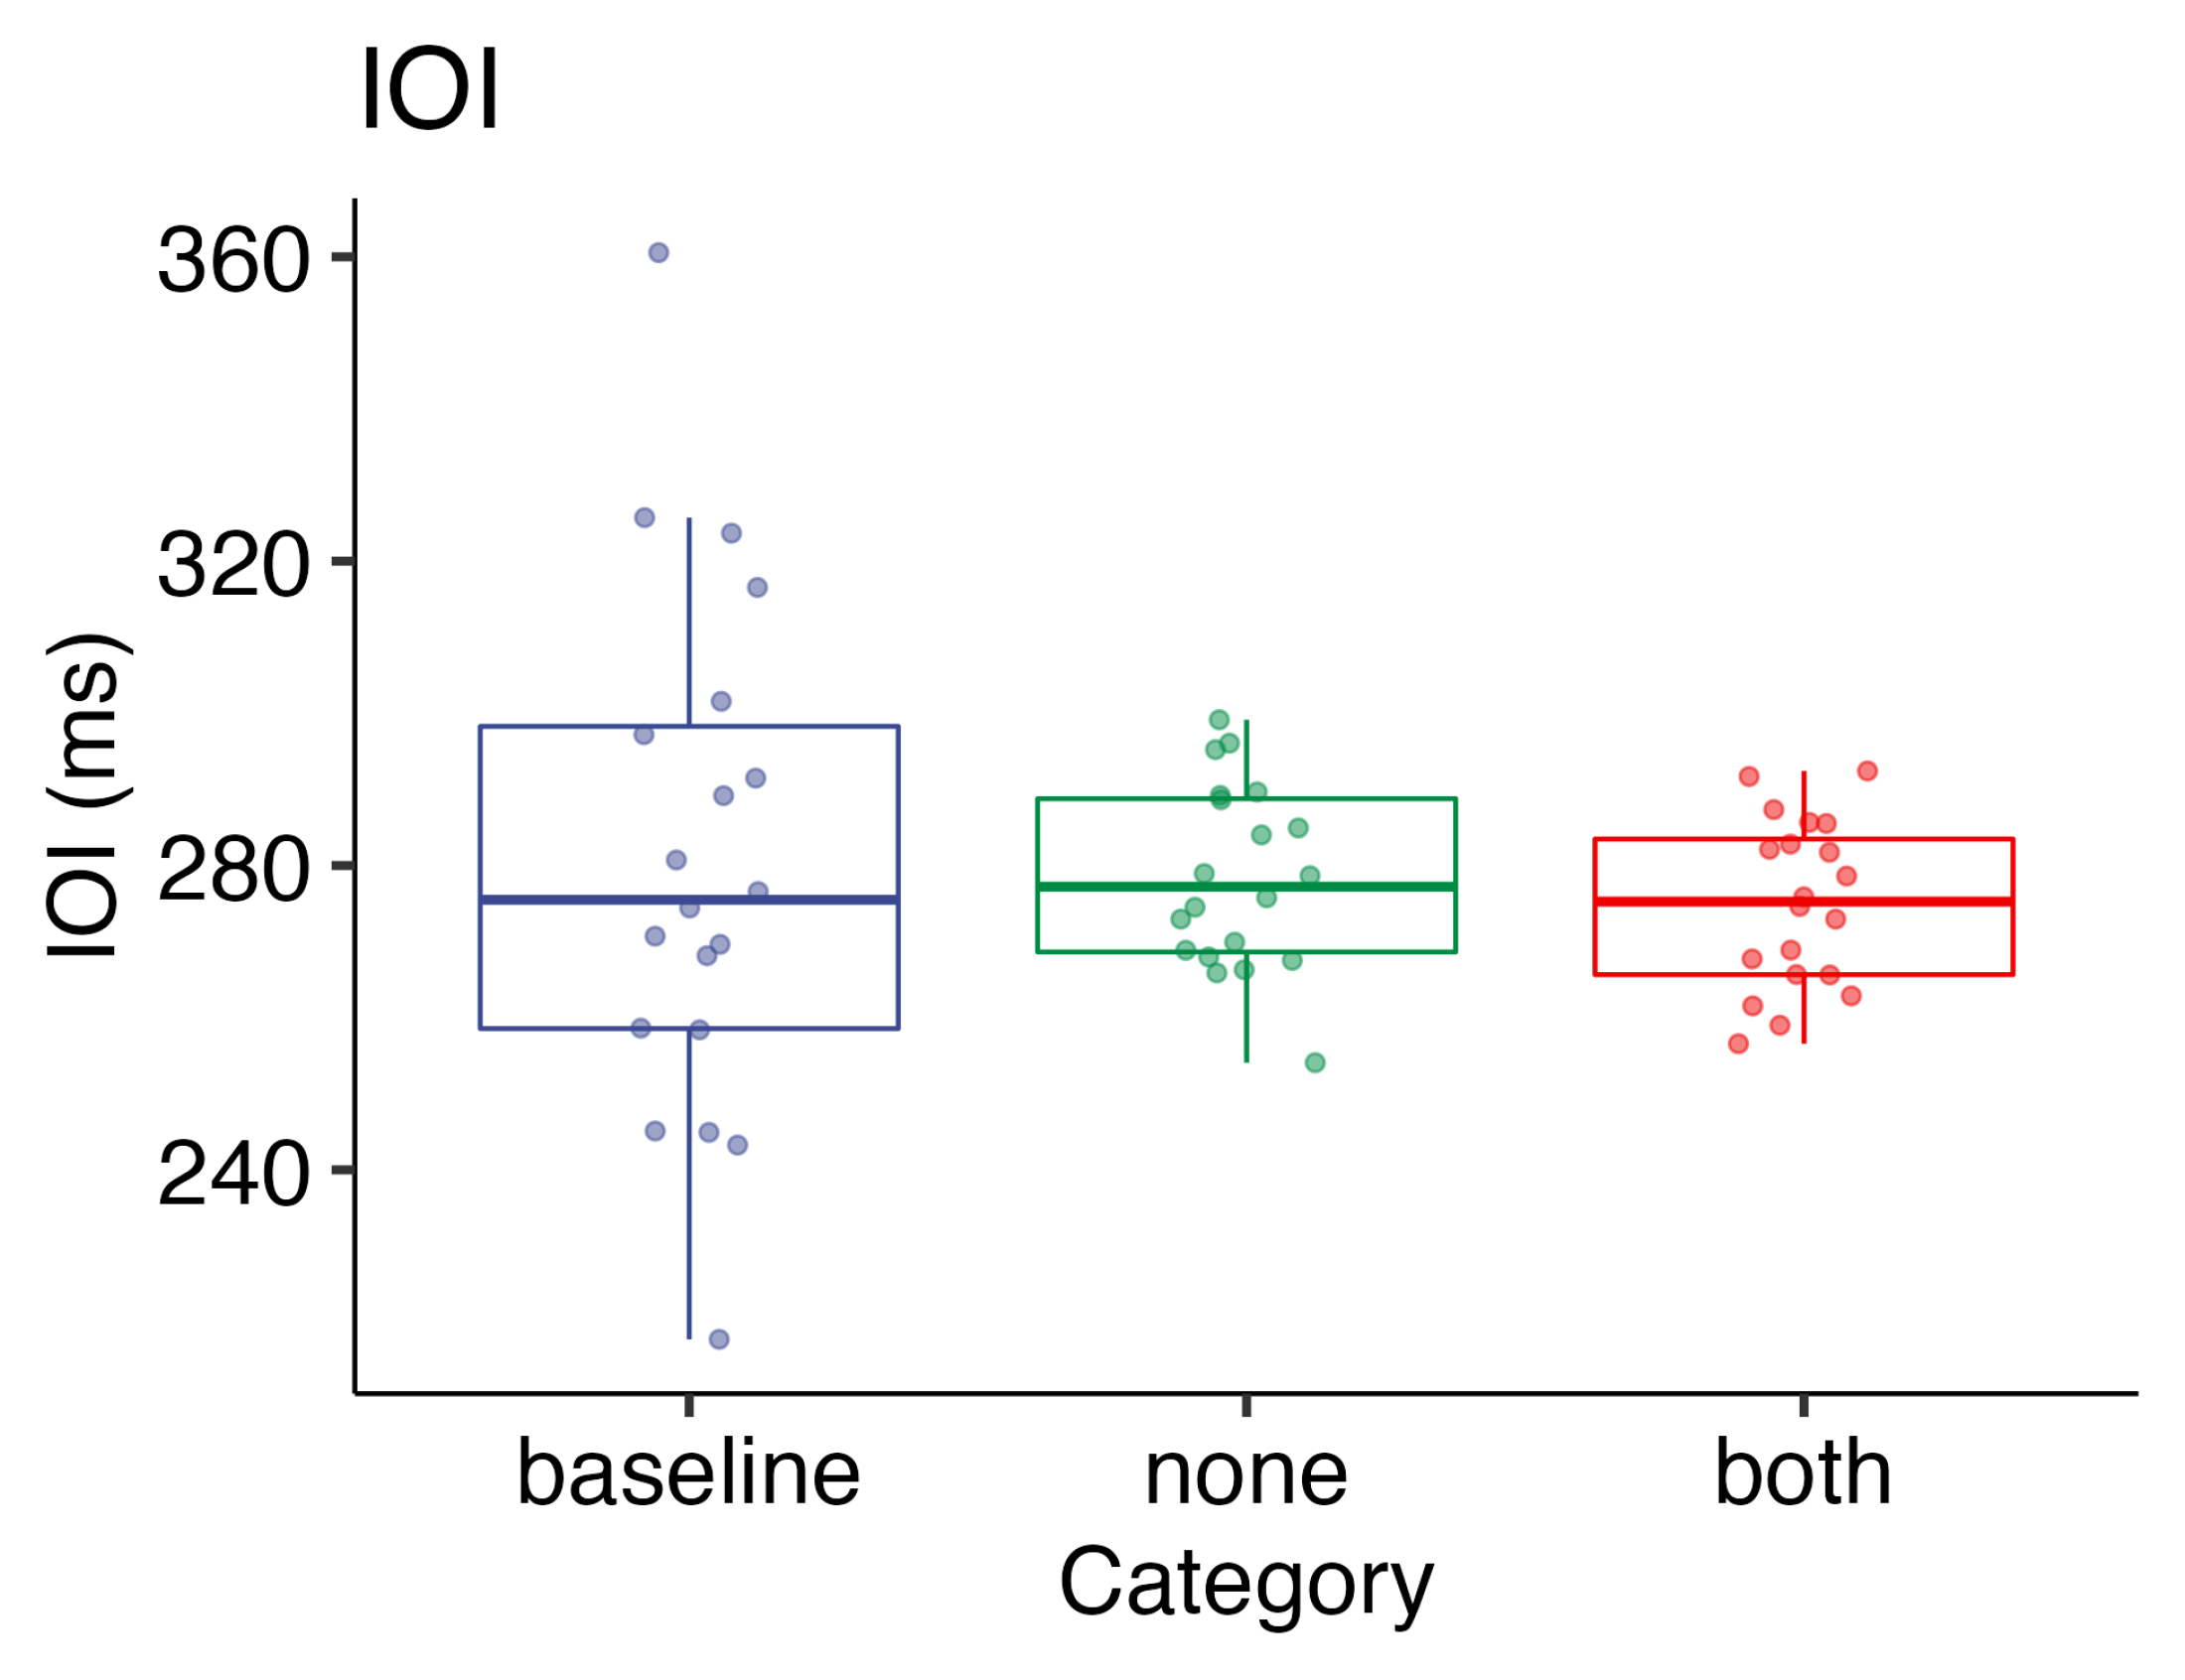
\includegraphics[width=1\linewidth]{manuscript_files/figure-latex/plot-ioi-2-1} \caption{\label{fig:ioi-2}Comparison with the baseline performance in terms of IOIs (ms). Each box indicates the IQR with the median, and whiskers extend to a maximum of 1.5 × IQR beyond the box.}\label{fig:plot-ioi-2}
\end{figure}

\begin{figure}
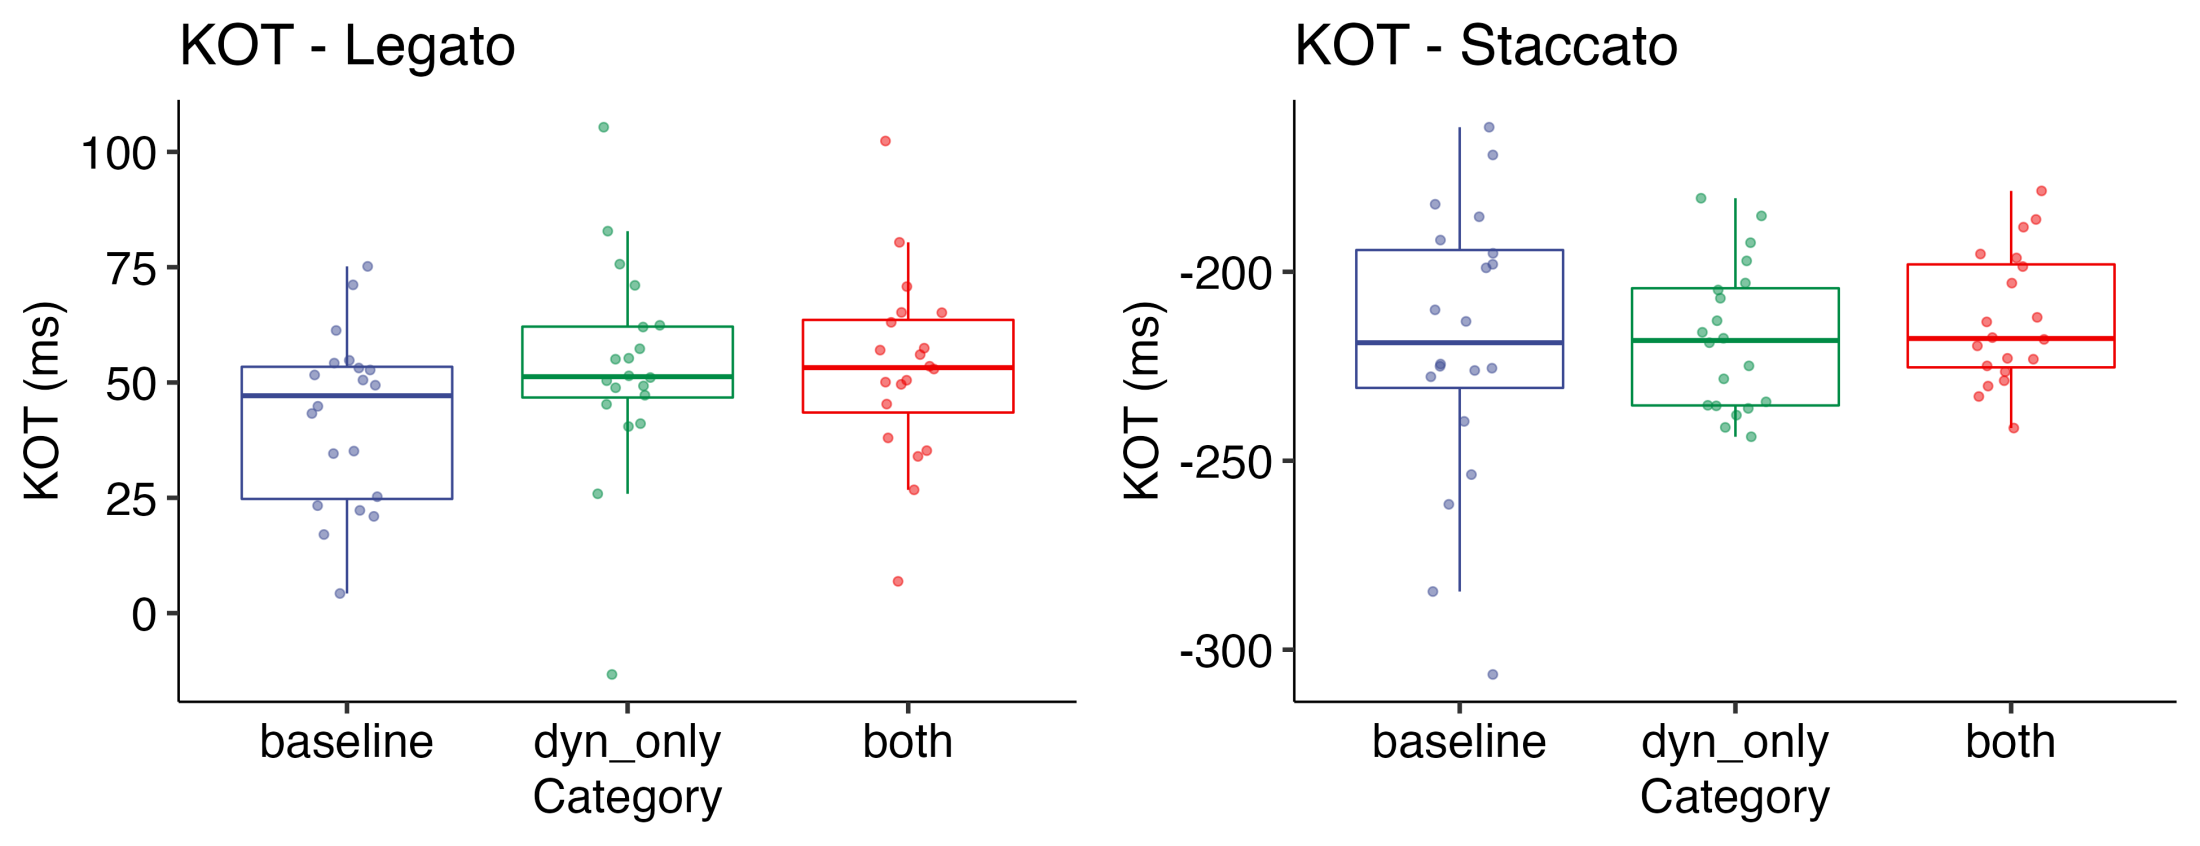
\includegraphics[width=1\linewidth]{manuscript_files/figure-latex/plot-kot-2-1} \caption{\label{fig:kot-2}Comparison with the baseline performance in terms of KOT(ms) for each subcomponent; legato (left) and staccato (right). Each box indicates the IQR with the median, and whiskers extend to a maximum of 1.5 × IQR beyond the box.}\label{fig:plot-kot-2}
\end{figure}

\begin{figure}
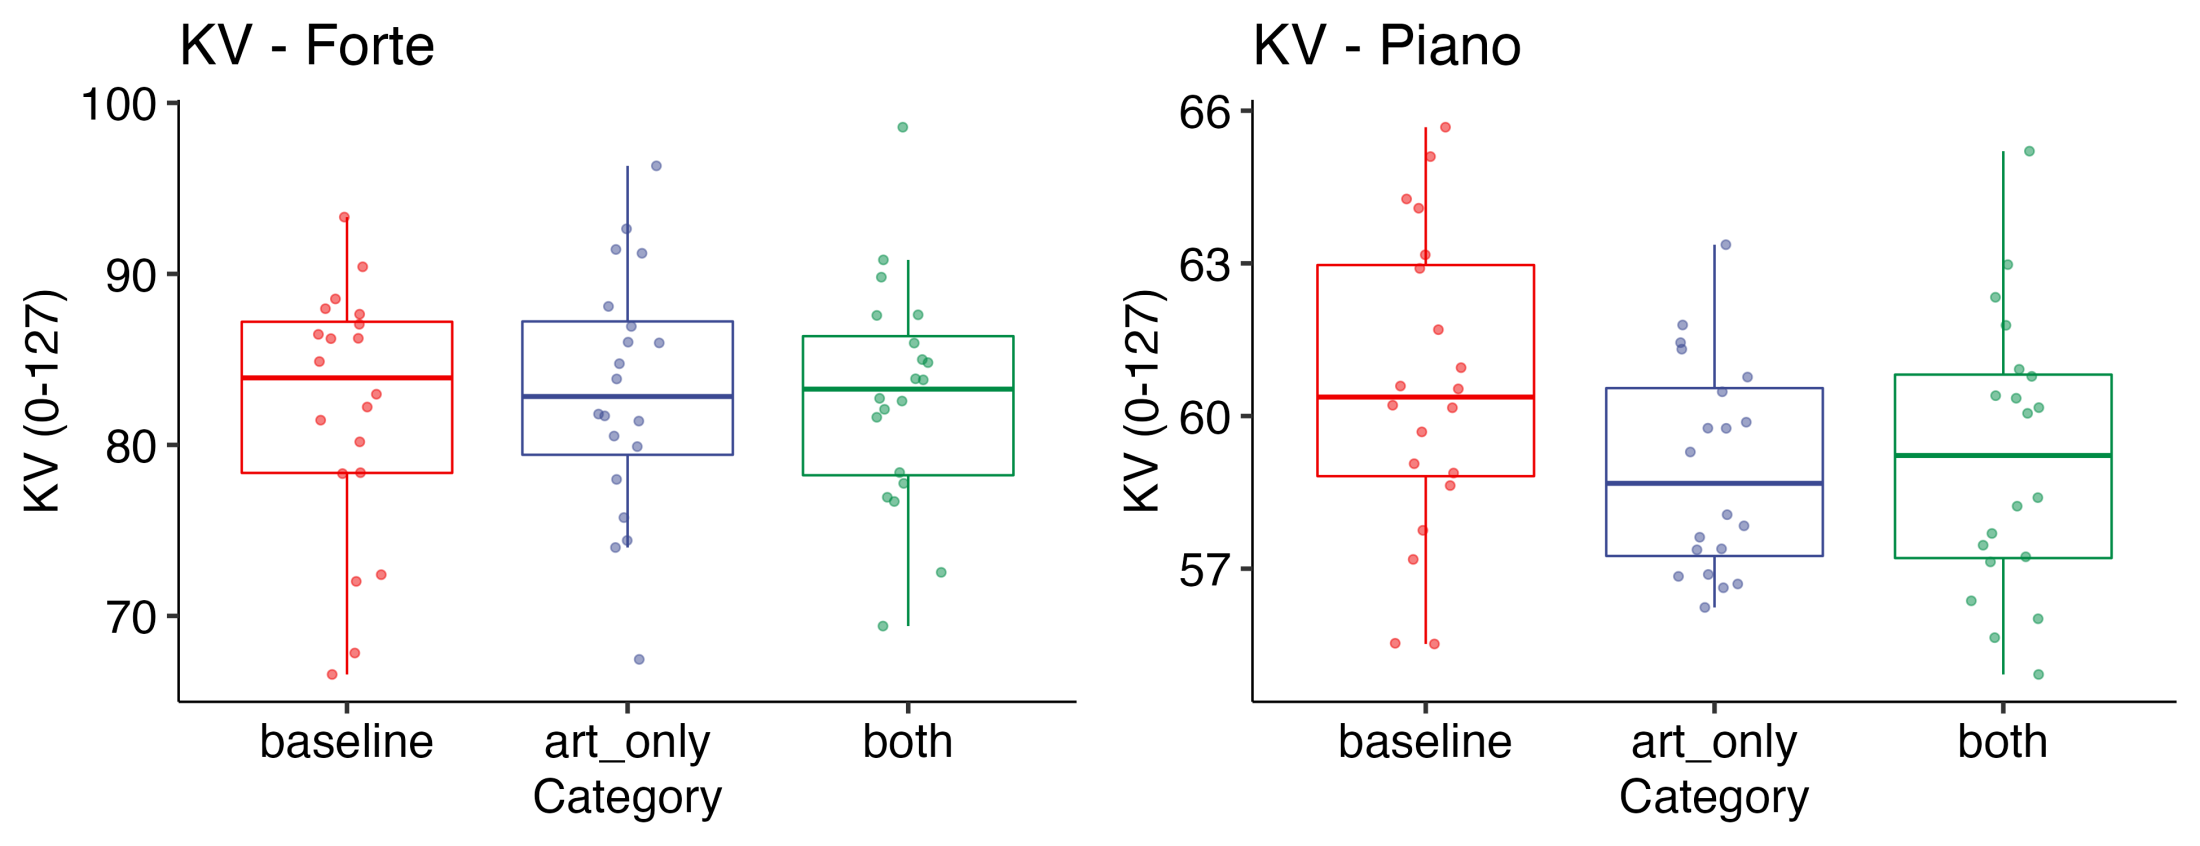
\includegraphics[width=1\linewidth]{manuscript_files/figure-latex/plot-vel-2-1} \caption{\label{fig:vel-2}Comparison with the baseline performance in terms of KV (0-127) for each subcomponent; forte (left) and piano (right). Each box indicates the IQR with the median, and whiskers extend to a maximum of 1.5 × IQR beyond the box.}\label{fig:plot-vel-2}
\end{figure}

\begin{figure}
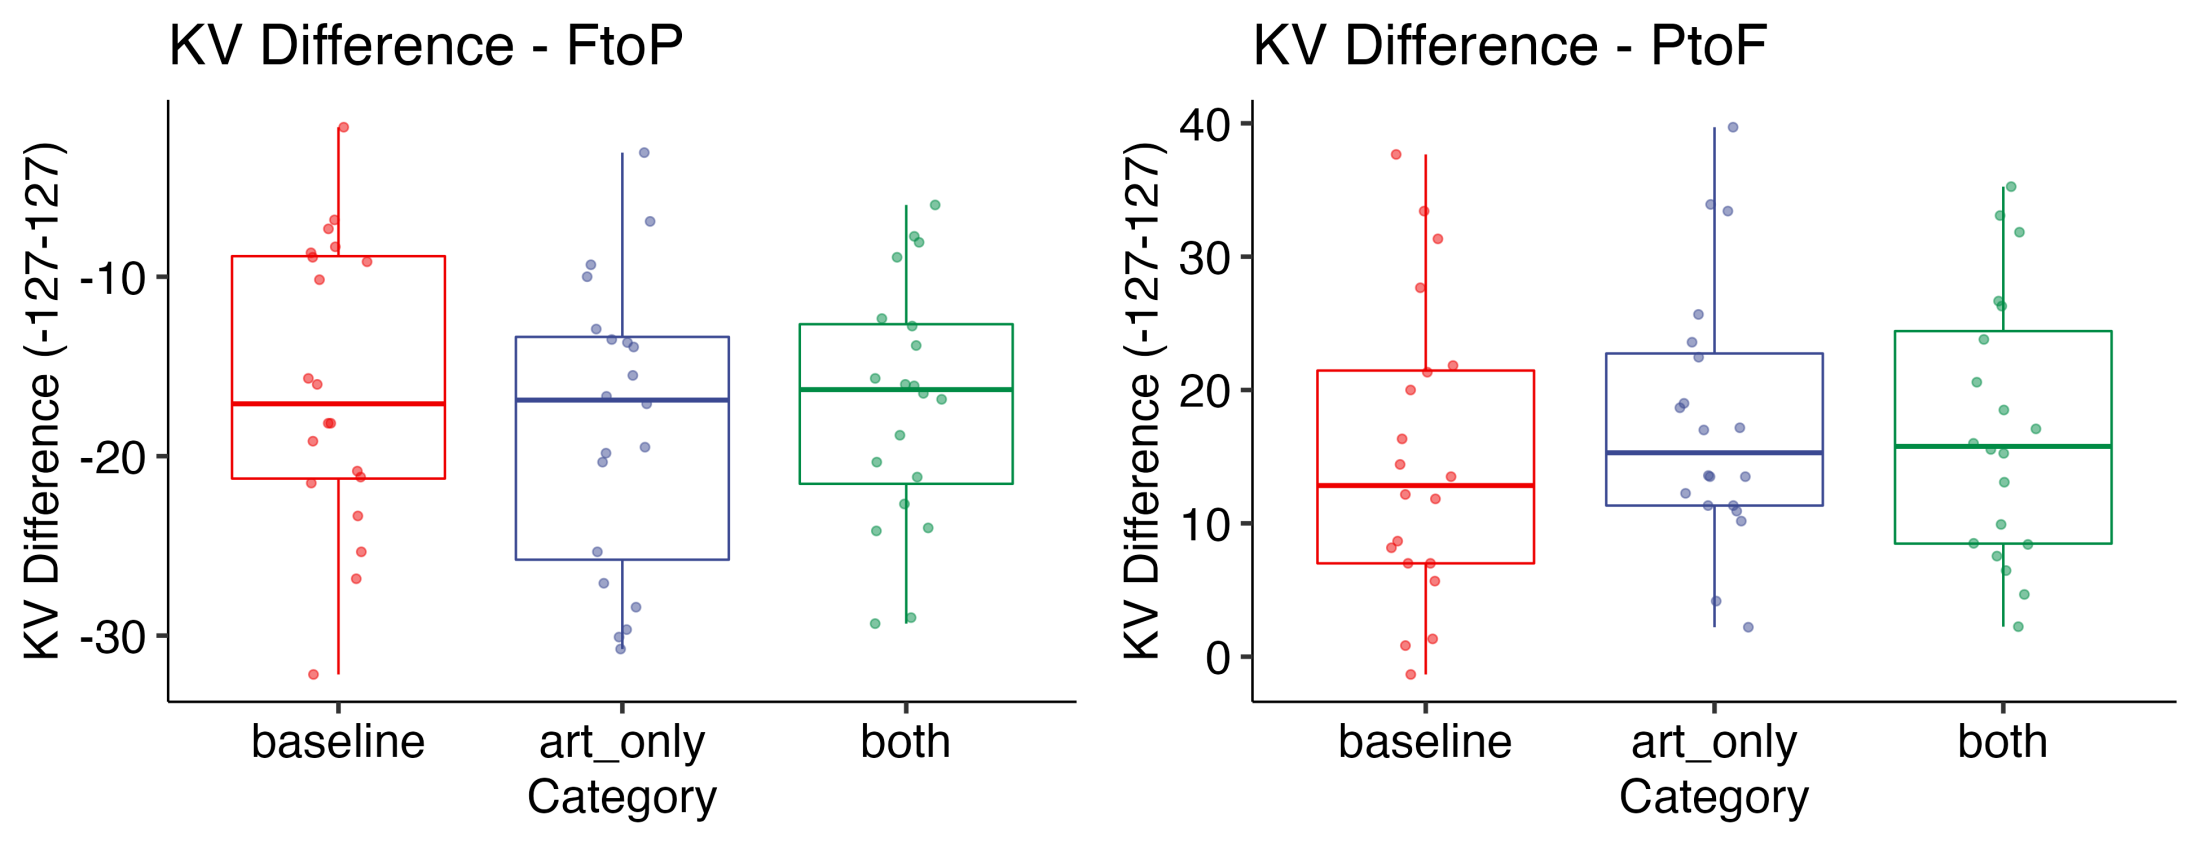
\includegraphics[width=1\linewidth]{manuscript_files/figure-latex/plot-vel-diff-2-1} \caption{\label{fig:vel-diff-2}Comparison with the baseline performance in terms of KV Difference (-127-127) for each subcomponent; forte to piano (left) and piano to forte (right). Each box indicates the IQR with the median, and whiskers extend to a maximum of 1.5 × IQR beyond the box.}\label{fig:plot-vel-diff-2}
\end{figure}

\hypertarget{discussion}{%
\section{Discussion}\label{discussion}}

The present study investigated whether and how expert pianists adapt their performance depending on the skill levels of students. We created artificial recordings to manipulate the skill levels by modifying the implementation of two musical expressive techniques (i.e., articulation and dynamics) notated on the sheet music. The recordings where the two techniques were implemented were supposed to replicate the performances of students with high skills. On the other hand, the recordings where none of the two techniques was implemented were supposed to replicate the performances of students with low skills. The recordings where either of the two techniques was implemented but the other was missing were equivalent to the performances of students with intermediate skills.

We found that expert pianists did not modulate their tempo (IOIs) depending on the skill levels of students. Even compared with the tempo of the baseline performance, they did not change their tempo either. These findings indicated that tempo was not employed specifically for teaching because tempo itself was relevant to neither articulation nor dynamics. Especially in music performance, it may not be an effective strategy to perform slowly as changing tempo might give another interpretation of music (e.g., expressive timing).

For KOT, expert pianists exaggerated legato and staccato when articulation was not implemented in the recordings. This is in line with our predictions that experts would exaggerate only the relevant aspects of the performance if a particular technique was missing in the recordings. However, we did not find significant results in terms of dynamics. Instead, we found that expert pianists produced softer piano when articulation was implemented in the recordings. Participants exaggerated piano only when there was no problem with regard to articulation in the recordings.

Overall, the results indicated that expert pianists seemed to prioritise the teaching of articulation. One possibility would be that articulation was more important for the piece we selected or the piece itself naturally invited some implementation of articulation. In our previous experiment, we observed most participants implemented articulation (particularly legato) when they were asked to perform the piece even when neither of articulation nor dynamics was notated on the sheet music. Therefore, it is possible that expert pianists were particularly sensitive to the lack of articulation in the recordings and trying to teach it. Another possibility is that dynamics modulations in the recordings were too subtle to be noticed by participants.

One of the limitations of the current study is that participants did not have an idea about what the ideal performance was. As some participants reported that ``(students had) very different interpretations of the melody'' or ``all kids played rhythmically correct'' in the questionnaire, it is plausible that the lack of articulation and/or dynamics might not have been perceived as errors. One solution would be to create a model performance where both articulation and dynamics was implemented and ask participants (expert pianists) to listen to it before starting the current experiment so that they can detect errors in the recordings.

The reason why participants considered different recording variations as interpretations rather than errors might stem from the fact that all the recordings did not include any pitch errors and performed the piece with the stable tempo. This was to make sure that we manipulated articulation and dynamics features of the recordings only. However, all the recordings might not have sounded like unskillful students were playing. In order to create more realistic unskillful performances, it might be useful to add some jitters to the tempo of the recordings we created, or to ask unskillful students to play the piece and extract the temporal feature of their performances.

Evidence from infant-directed action research has shown that caregivers are sensitive to the infants' skill levels and modified their demonstration according to infants' abilities to perform a motor task (Fukuyama et al., 2015). In the current experiment, expert pianists needed to perform in the absence of actual students. Future research should investigate how expert pianists and students dynamically interact in a situation where they can communicate as a naturalistic lesson and examine how the performance of expert pianists and that of students are related.

\hypertarget{references}{%
\section{References}\label{references}}

\hypertarget{acknowledgement}{%
\section*{Acknowledgement}\label{acknowledgement}}
\addcontentsline{toc}{section}{Acknowledgement}

\hypertarget{refs}{}
\begin{CSLReferences}{1}{0}
\leavevmode\vadjust pre{\hypertarget{ref-fukuyama_2015}{}}%
Fukuyama, H., Qin, S., Kanakogi, Y., Nagai, Y., Asada, M., \& Myowa-Yamakoshi, M. (2015). Infant's action skill dynamically modulates parental action demonstration in the dyadic interaction. \emph{Developmental Science}, \emph{18}(6), 1006--1013. \url{https://doi.org/10.1111/desc.12270}

\end{CSLReferences}


\end{document}
